\chapter{Protocol Trends in CAIDA Traces}\label{adx:caida-traffic}
In an earlier version of the work in \cref{chap:ddos-rl} which we chose to submit to the EuroS\&P '19 conference\sidenote{Rejected, of course.}, I backed up my analysis of the shortcomings of \emph{Marl}~\parencite{DBLP:journals/eaai/MalialisK15}---i.e., that \gls{acr:tcp} traffic is both dominant and negatively impacted---by referencing a study from \Textcite{DBLP:conf/saint/ZhangDJC09} which suggested that \gls{acr:tcp} traffic was most prevalent in packet and byte counts for Internet traffic.
In addition to other feedback mostly unactionable short of working for a hyper-giant/-scaler operator, Reviewer 1 raised the challenge that:
\begin{quote}
\noindent
The statistics borrowed from [\cite{DBLP:conf/saint/ZhangDJC09}] are 10 years old by now; I imagine that the Internet traffic has changed significantly by then due to streaming services and new protocol developments.
\end{quote}
So-challenged---in spite of the fact that streaming video is most often \gls{acr:dash}-based (i.e., carried over \gls{acr:http}, so \gls{acr:tcp}) and that prominent new protocols are themselves congestion-aware (e.g., QUIC)\sidenote{This overview might read rather like a polemic against said review---this is merely an attempt to add enough context to make an otherwise dry appendix a tad more entertaining.}---I carried out a high-level analysis of the \gls{acr:caida} 2018 passive traces dataset~\parencite{caida-2018-passive} while the school's network infrastructure was otherwise knocked out due to a malware incursion.
Simply put, the aim was to see whether the same observations held: that congestion-aware traffic outnumbered congestion-unaware traffic, in either packets or bytes, on a reasonable view of Internet traffic.
Analysis of the these datasets shows that in an Internet backbone link belonging to a Tier 1 \gls{acr:isp}, congestion-aware traffic makes up at least \qtyrange{73}{82}{\percent} of packets, corresponding to \qtyrange{77}{84}{\percent} of data volume.

%Detail and explain the stuff in that repo here.\gls{acr:caida}~\parencite{caida-2018-passive}

\section{Dataset description}
The \gls{acr:caida} 2018 passive traces are a set of anonymised Pcap files captured over a \qty{1}{\hour} period each month from the \emph{equinix-nyc} monitor (observed March--December from 1300--1400 UTC\sidenote{Depending on daylight savings time, these endpoints fall in UTC-\{4,5\}$\leftrightarrow$UTC-3 respectively. For most data points at NYC, this corresponds to 0900--1000 EDT.}), subdivided into \qty{1}{\minute} traces.
Source and destination \gls{acr:ip} addresses are anonymised in a prefix-preserving manner.
Captured packets have been stripped of their payload data, and remaining headers are accompanied by \unit{\micro\second}-precise timestamps.
Traces are captured over both directions for a monitored Internet backbone link (\qty{9953}{\mega\bit\per\second}, Tier 1 \gls{acr:isp}) between New York and Sao Paulo: direction A runs from Sao Paulo to New York, while direction B is the reverse of this.
The official description contains greater detail~\parencite{caida-2018-passive}.

\section{Data processing methodology}
Traces are examined at a packet-level granularity, and IPv4 and v6 packets are classified based on their L3/L4 header fields:
\begin{description}
	\item[\gls{acr:tcp}] Packets with a \emph{protocol} or \emph{next header} value of \mintinline{rust}|0x06|.
	\item[\gls{acr:udp} (QUIC)] Packets with a \emph{protocol} or \emph{next header} value of \mintinline{rust}|0x11|, and a source or destination port of 80 or 443.\sidenote{This category is not necessarily definitive, and is based on then-current descriptions from Google on how Chrome was initiating QUIC sessions. These packets aren't \emph{provably} QUIC, but are speculated to be so. \gls{acr:caida}'s payload stripping removes any bytes past the \gls{acr:udp} header, making this impossible to conclusively verify.}
	\item[\gls{acr:udp} (Non-QUIC)] Packets with a \emph{protocol} or \emph{next header} value of \mintinline{rust}|0x11| and any other source and/or destination ports. This includes \gls{acr:udp} packets whose ports had been truncated or removed entirely due to \gls{acr:ip} options.
	\item[Other] All other packets.
\end{description}
For each one hour period, I store individual packet counts and payload bytes for each category in \mintinline{rust}|u64|s.
Category counts from sub-traces in the same month are summed together, and once totalled I locally store the counts and proportions of each traffic class (bytes and packets).
This is performed for directions A and B separately (\emph{Dir A}, \emph{Dir B}), which are then combined appropriately (\emph{Both}).

\paragraph{Categorisation}
%These classifications are grouped for easier analysis.
Congestion-aware packets are defined as those who are either \emph{\gls{acr:tcp}} or \emph{\gls{acr:udp} (QUIC)}.
\gls{acr:udp} packets (\emph{QUIC} and \emph{Non-QUIC}) are also combined into their own category.

While this analysis ignores other congestion-aware protocols and (cannot be certain on the proportion of QUIC traffic due to the trace data format), this allows us to establish a sensible lower bound on their proportion in the network.
Assuming there is no ongoing \gls{acr:tcp} replay-driven attack in any trace, we can state that the \emph{lower bound} on congestion-aware traffic lies between $\operatorname{\%}(\mathit{TCP})$ and $\operatorname{\%}(\mathit{TCP} + \mathit{QUIC})$.
Similarly, the remainder of these quantities from \num{1.0} gives us the range of an \emph{upper} bound on congestion-unaware traffic.

\paragraph{Implementation}
The above analysis program was implemented in Rust by incrementally streaming, unzipping, and parsing Gzipped packet captures using the \emph{reqwest} library.
Individual trace files are mined from the main directory page, which is served as HTML.
As network access was the limiting factor in handling this data, these are processed sequentially and in-memory due to the large size of each pcap file (totalling $\mathcal{O}\left(\unit{\tebi\byte}\right)$).

\section{Results}
\Cref{fig:caida-ca} shows that congestion-aware traffic makes up at least \qtyrange{73}{82}{\percent} of packets, corresponding to \qtyrange{77}{84}{\percent} of data volume when considering both transit directions.
In \emph{direction A} (Sao Paulo$\rightarrow$New York) we can see byte volumes are far greater (\qtyrange{85}{92}{\percent}), while packet counts are roughly symmetric.
These trends are effectively replicated for \gls{acr:tcp} traffic (\cref{fig:caida-tcp}).
The main takeaway is that in both byte volume and proportion of sent packets, \gls{acr:tcp} still routinely makes up the majority of Internet traffic, and both are higher still for congestion-aware transports.

In the case of \gls{acr:udp} traffic including QUIC (\cref{fig:caida-udp}), packet counts are again fairly symmetrical---ranging over \qtyrange{15}{26}{\percent} when considering the aggregate of both directions.
Although \gls{acr:udp} traffic has a lower packet prevalence in \emph{Dir B}, it consistently has a higher proportion of seen bytes flowing from New York$\rightarrow$Sao Paulo.

Supposed QUIC packets do not have much prevalence---particularly in \emph{Dir B}
(\cref{fig:caida-quic}).
We do observe some spikes in activity in \emph{Dir A} ranging over July--September, in \qty{3.6}{\percent} of packets and \qty{4.5}{\percent} of carried bytes.
This falls a little below other estimates of the protocol's prevalence; for instance, \Textcite{DBLP:conf/pam/RuthPDH18} found that it occupied some \qtyrange{2.6}{9.1}{\percent} of network traffic across another Tier-1 \gls{acr:isp} and an \gls{acr:ixp}.
The time of measurement (early-to-mid morning at both endpoints) may be a factor here, as QUIC's main purpose at this time was for video transit rather than the basis of \gls{acr:http}/3~\parencite{ietf-quic-http-34}.
The main body type---video---does neatly explain why it occupies a larger share of carried bytes than packets.

\newlength{\caidafig}
\setlength{\caidafig}{1.0\linewidth}

\begin{figure}
	\centering
	\begin{subfigure}{\linewidth}
		\centering
		\resizebox{\caidafig}{!}{
			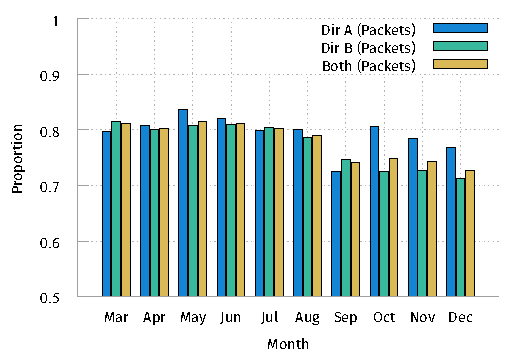
\includegraphics{plots/caida/ca-monthly-pres}
		}
		\caption{Congestion-aware packets.}
	\end{subfigure}
	\begin{subfigure}{\linewidth}
		\centering
		\resizebox{\caidafig}{!}{
			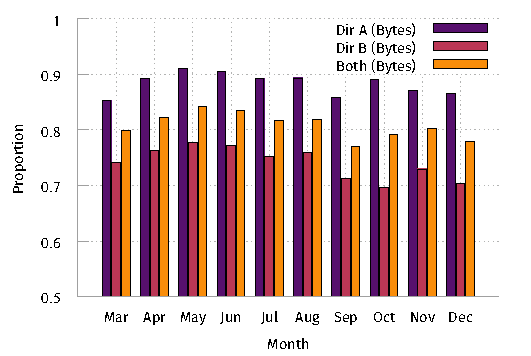
\includegraphics{plots/caida/ca-monthly-pres-bytes}
		}
		\caption{Congestion-aware byte volume.}
	\end{subfigure}
	\caption{Proportional counts and byte volume of congestion-aware traffic.\label{fig:caida-ca}}
\end{figure}

\begin{figure}
	\centering
	\begin{subfigure}{\linewidth}
		\centering
				\resizebox{\caidafig}{!}{
			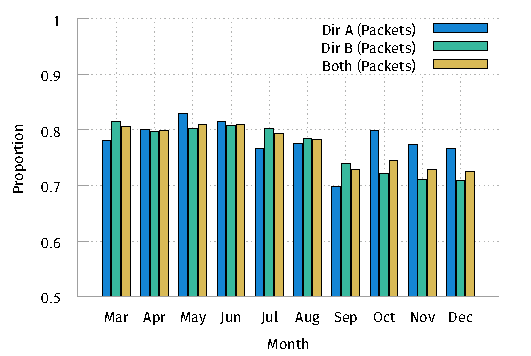
\includegraphics{plots/caida/tcp-monthly-pres}
					}
		\caption{\gls{acr:tcp} packets.}
	\end{subfigure}
	\begin{subfigure}{\linewidth}
		\centering
				\resizebox{\caidafig}{!}{
			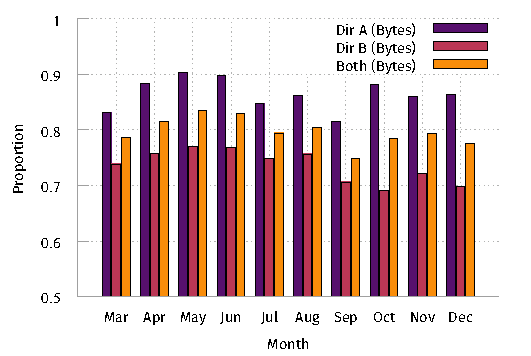
\includegraphics{plots/caida/tcp-monthly-pres-bytes}
					}
		\caption{\gls{acr:tcp} byte volume.}
	\end{subfigure}
	\caption[Proportional counts and byte volume of TCP traffic.]{Proportional counts and byte volume of \gls{acr:tcp} traffic.\label{fig:caida-tcp}}
\end{figure}

\begin{figure}
	\centering
	\begin{subfigure}{\linewidth}
		\centering
				\resizebox{\caidafig}{!}{
			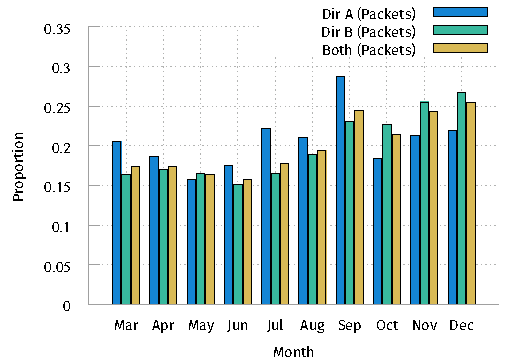
\includegraphics{plots/caida/udp-monthly-pres}
					}
		\caption{\gls{acr:udp} packets.}
	\end{subfigure}
	\begin{subfigure}{\linewidth}
		\centering
				\resizebox{\caidafig}{!}{
			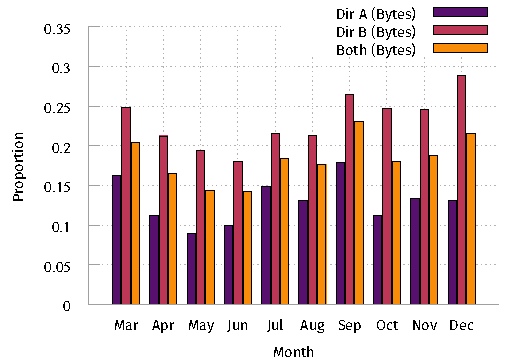
\includegraphics{plots/caida/udp-monthly-pres-bytes}
					}
		\caption{\gls{acr:udp} byte volume.}
	\end{subfigure}
	\caption[Proportional counts and byte volume of UDP traffic.]{Proportional counts and byte volume of \gls{acr:udp} traffic.\label{fig:caida-udp}}
\end{figure}

\begin{figure}
	\centering
	\begin{subfigure}{\linewidth}
		\centering
				\resizebox{\caidafig}{!}{
			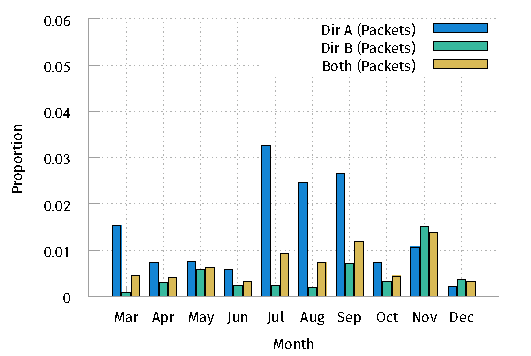
\includegraphics{plots/caida/quic-monthly-pres}
					}
		\caption{QUIC packets.}
	\end{subfigure}
	\begin{subfigure}{\linewidth}
		\centering
				\resizebox{\caidafig}{!}{
			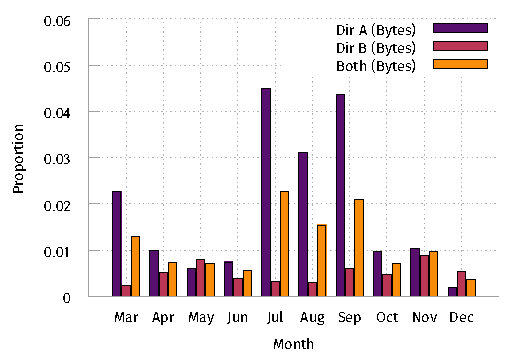
\includegraphics{plots/caida/quic-monthly-pres-bytes}
					}
		\caption{QUIC byte volume.}
	\end{subfigure}
	\caption[Proportional counts and byte volume of UDP (QUIC) traffic.]{Proportional counts and byte volume of \gls{acr:udp} (QUIC) traffic.\label{fig:caida-quic}}
\end{figure}